%File: formatting-instructions-latex-2023.tex
%release 2023.0
\documentclass[letterpaper]{article} % DO NOT CHANGE THIS
\usepackage{aaai23}  % DO NOT CHANGE THIS
\usepackage{times}  % DO NOT CHANGE THIS
\usepackage{helvet}  % DO NOT CHANGE THIS
\usepackage{courier}  % DO NOT CHANGE THIS
\usepackage[hyphens]{url}  % DO NOT CHANGE THIS
\usepackage{graphicx} % DO NOT CHANGE THIS
\graphicspath{{images/}}

\urlstyle{rm} % DO NOT CHANGE THIS
\def\UrlFont{\rm}  % DO NOT CHANGE THIS
\usepackage{natbib}  % DO NOT CHANGE THIS AND DO NOT ADD ANY OPTIONS TO IT
\usepackage{caption} % DO NOT CHANGE THIS AND DO NOT ADD ANY OPTIONS TO IT
\frenchspacing  % DO NOT CHANGE THIS
\setlength{\pdfpagewidth}{8.5in}  % DO NOT CHANGE THIS
\setlength{\pdfpageheight}{11in}  % DO NOT CHANGE THIS
%
% These are recommended to typeset algorithms but not required. See the subsubsection on algorithms. Remove them if you don't have algorithms in your paper.
\usepackage{algorithm}
\usepackage{algorithmic}
\usepackage{bm}
\usepackage{amsmath}
\usepackage{todonotes}
%
% These are are recommended to typeset listings but not required. See the subsubsection on listing. Remove this block if you don't have listings in your paper.
\usepackage{newfloat}
\usepackage{listings}
\DeclareCaptionStyle{ruled}{labelfont=normalfont,labelsep=colon,strut=off} % DO NOT CHANGE THIS
\lstset{%
	basicstyle={\footnotesize\ttfamily},% footnotesize acceptable for monospace
	numbers=left,numberstyle=\footnotesize,xleftmargin=2em,% show line numbers, remove this entire line if you don't want the numbers.
	aboveskip=0pt,belowskip=0pt,%
	showstringspaces=false,tabsize=2,breaklines=true}
\floatstyle{ruled}
\newfloat{listing}{tb}{lst}{}
\floatname{listing}{Listing}
%
% Keep the \pdfinfo as shown here. There's no need
% for you to add the /Title and /Author tags.
\pdfinfo{
/TemplateVersion (2023.1)
}

\setcounter{secnumdepth}{0} %May be changed to 1 or 2 if section numbers are desired.

\title{Detecting Offensive Language in Tweets with Attention-fused Text and User Embeddings}
\author {
    % Authors
    Viha Gupta,\textsuperscript{\rm 1}
    Casey Primel\textsuperscript{\rm 1}
}
\affiliations {
    % Affiliations
    \textsuperscript{\rm 1} Dept. of Computer Science\\
    vg2237@nyu.edu, ctp219@nyu.edu
}



\begin{document}

\maketitle

\begin{abstract}
    Transformer-based models have come to dominate natural language processing tasks including difficult problems in computational linguistics such as semantic and sentiment analysis. One application for these models is automated content moderation for social media platforms where they can be deployed to flag and remove abusive or harmful content. In the context of offensive language detection, recent research demonstrates that the performance of such models can be improved by incorporating information about the communities where that content is produced. For our project, we experiment with a novel technique for fusing community structure features and text features to classify offensive language in an end-to-end model via attention mechanisms. We incorporate a "corrected" procedure for computing attention on graph-structured data to produce our user embeddings and a better performing bidirectional encoder for our text embeddings into an existing architecture. Our model achieves a mean F1 score of 0.8936 barely outperforming our baseline model by 0.0009. Further, our ablation analysis demonstrates that attention fusion tends towards diminishing returns as the underlying embeddings become more expressive. Our code is available at \url{https://github.com/guptaviha/GF-OLD}.
\end{abstract}

\section{Introduction}

Content moderation is a pressing concern for online communities. For over a decade, automated systems have been employed to identify abusive behaviors and offensive language in user-generated content. Early systems relied on hand-crafted rules to extract linguistic features from textual data. Such rule-based systems have largely been replaced by neural network-based systems that can identify more subtle patterns in users' linguistic behaviors. However, research has shown that textual features are not always sufficient for identifying the nature of user-generated content. The rise of social media and the corollary ability to query the social graphs formed by users' activity opened up a rich data source for constructing the requisite context. The remaining question is how to most effectively provide such context from the available data. Our project focuses on one solution in the context of deep learning for offensive language detection in Twitter datasets: the fusion of text and user embeddings in an end-to-end model via attention mechanisms.

Recent work exploring the application of deep learning for offensive language detection in tweets can be divided into two different approaches. The first approach focuses solely on text data (e.g., tweets) and the use of pre-trained language models fine-tuned for this domain-specific task. Architectures centered around bidirectional encoder representations from transformers (BERT) have come to dominate this approach. For instance, \citet{liu2019-nuli} uses a pre-trained BERT model fine-tuned for only 3 epochs achieving an F1 score of 0.7826. \citet{Barbieri2020} surpass this score by retraining a RoBERTa-base model achieving an F1 score of 0.816.

The second approach combines text data with information about users and community structure. Typically, this involves training two models: a deep learning model from which user embeddings can be extracted and a classification model that takes as input a text representation and the user embeddings. \citet{qian-etal-2018-leveraging} and \citet{Mishra2019} are recent exemplars of this approach. \citet{qian-etal-2018-leveraging} train a bidirectional long-short term memory network (Bi-LSTM) to produce an intra-user representation based on a users' historical behavior and a reinforced Bi-LSTM network to selectively pull inter-user representation based on similar tweets. In this case, the intra-user representations are learned prior to the training of the reinforced Bi-LSTM network. \citet{Mishra2019} train a graph convolutional network (GCN) on a heterogeneous graph of users and tweets. The output of the first layer of the GCN is then used as input, along with a bag-of-words representation of the text data for a logistic regression model. \citet{qian-etal-2018-leveraging} and \citet{Mishra2019} achieve an F1 score of 0.774 and 0.854, respectively.

\citet{Miao2022} introduce a method for learning user and text embeddings concurrently and fusing them together before via attention mechanisms. \citet{Miao2022} derive their user embeddings from a graph attention network (GAT) trained on a homogenous social graph of users and the follower relationships between them. Text embeddings are taken from a pre-trained BERT model. These embeddings are then concatenated and fused via attention mechanisms before being passed along to a feedforward classification layer. \citet{Miao2022}'s end-to-end model, which serves as the starting point for our project, achieves a mean F1 score of 0.8994.

The following report describes our experiments with attention fusion in an end-to-end model for offensive language detection. We first evaluate possible improvements to the graph attention and bidirectional encoder modules. We find that introducing a "corrected" implementation of graph attention and a retrained RoBERTa model leads to a marginal improvement in the end-to-end model increasing the mean F1 score by 0.0009 from our baseline of 0.8927 to 0.8936. Our ablation analysis demonstrates that attention fusion tends towards diminishing returns as the underlying embeddings become more expressive.

\section{Methodology}

The aim of this project is to evaluate attention fusion as a means of combining text and community structure features. In practical terms, our first objective was to replicate the results of \citet{Miao2022}. With this as our baseline, we then attempted to surpass the baseline by incorporating modules which, when evaluated in isolation, outperformed the modules used by \citet{Miao2022} in their end-to-end model. Simply put, if more effective base modules were incorporated, then we expect attention fusion would carry those improvements forward to the end-to-end model.

In the rest of this section, we introduce our dataset, describe the architecture of the end-to-end model and our modifications to it. 

\subsection{Dataset and preprocessing}

For this project, we use the English-language dataset collected, labelled and made publicly available on GitHub by \citet{Miao2022}.\footnote{\url{https://github.com/mzx4936/GF-OLD-Dataset}} The data was obtained via the Twitter API\footnote{https://developer.twitter.com/en/docs/twitter-api} and contains data from 1,260 users and 12,780 of their tweets posted between January 2018 and March 2021. The dataset also captures the social community in terms of the follower-network between these users with 8,877 such relationships. Unlike other Twitter datasets, \citet{Miao2022} construct a dataset to preserve community structures and better reflect real-world distribution of offensive language. They accomplish this by constructing a lexicon of topic-related words rather than offensive words from which they then query for users and their first- and second-order friends whose tweets are also collected. The result is a dataset more reflective of real-world conditions where the ratio of offensive tweets is 7.90\%, i.e., 1,009 out of the 12,780 total.

To represent the social graph, the users and relationship data are used to construct a graph with the users represented by nodes and the follower relationships represented by edges. Drawing on the work of \citet{Mishra2019}, \citet{Miao2022} use the users' historical behavior to represent the propensity of the user to post offensive language. The number of tweets labelled non-offensive and offensive in the training data are used to describe users' historical behavior, i.e., the number of non-offensive tweets and the number of offensive tweets from the training data made by a user are each set as node attributes.

Several text preprocessing steps are taken to prepare the raw text data: emojis are converted to words with similar meanings using third-party libraries\footnote{emoji (\url{https://github.com/carpedm20/emoji}) and ekphrasis (\url{https://github.com/cbaziotis/ekphrasis}).}, URLs replaced with "\textit{http}", hashtags segmented into phrases, and text like user references, dates and email addresses are converted into uniform placeholders, e.g., "\textit{@anonymous2134}" becomes "\textless\textit{user}\textgreater".

\subsection{Model architecture}

\begin{figure}
    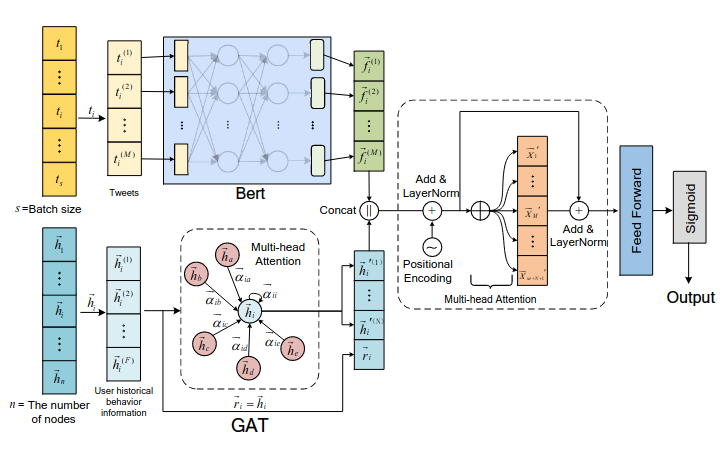
\includegraphics[width=\linewidth]{architecture_diagram.png}
    \caption{End-to-end offensive language detection model \citep{Miao2022}.}
\end{figure}

We follow \citet{Miao2022} in using a graph attention network for learning user embeddings, a language model for deriving the text embeddings and attention mechanisms for fusing user and text embeddings together before passing the fused embeddings to a classification layer. However, we introduce a modification to GAT proposed by \citet{Brody2021} for computing what they call \textit{dynamic attention}. In addition, rather than using text embeddings from BERT, we use two variations of RoBERTa language model: the base RoBERTa model \citep{Devlin2018} and a variant pre-trained on tweets and fine-tuned for offensive language detection \citep{Barbieri2020}.\footnote{\url{https://huggingface.co/cardiffnlp/twitter-roberta-base-offensive}}

All the models discussed here use Adam optimizer \citep{Kingma2014} and focal loss function \citep{lin2017focal}, a modified cross entropy loss designed for dealing with class imbalance. It introduces a scaling factor $(1-p_t)^\gamma$ such that setting $\gamma > 0$ reduces the relative loss for easy examples and puts more emphasis on hard to classify examples. The function can be written

$$
FL(p_t) = \alpha \cdot (1 - p_t)^\gamma \log{p_t}
$$

where $p_t = \begin{cases} p, & \text{if } y =1 \\ 1-p, & \text{otherwise}  \end{cases}$, i.e., the magnitude of the estimated probabilty irrespective of the class label. In the special case where $\gamma=0$, the focal loss function simplifies to cross entropy loss.

\subsubsection{Transformer-based language models}

As discussed above, \citet{Miao2022}'s end-to-end model uses BERT \citep{Devlin2018}, a transformer-based language model designed for easy fine-tuning on downstream tasks\citep{Devlin2018}. \citet{Liu2019} found BERT to be significantly understrained and presented a set of improved BERT design choices and training strategies. The product of \citet{Liu2019}'s improved recipe, roBERTa, includes: (1) training the model longer, with bigger batches (8K), over more data; (2) removing the Next Sentence Prediction (NSP) loss to impove downstream tasks which require reasoning about the relationsps between sentence pairs; (3) training on longer full-length sequences; and, (4) dynamically changing the masking pattern applied to the training data compared to the single static masking performed in BERT. A byproduct of (2) is particularly important for the present context: cutting NSP makes it more suitable for downstream tasks where "sentence" inputs are not part of a larger text, e.g., tweets.

We incorporate RoBERTa into our end-to-end model as a replacement for BERT in \citet{Miao2022}'s end-to-end model keeping the model hyperparameters the same. We try both a base RoBERTa model and a variant fine-tuned for the specific task of offensive language detection in tweets, RoBERTa-RT \citep{Barbieri2020}. RoBERTa-RT retrains RoBERTa-base model on a 60 million Twitter corpus. We use RoBERTa-RT fine-tuned specifically for offensive language detection.\footnote{See RoBERTa-RT-base for Offensive Language Identification. \url{https://huggingface.co/cardiffnlp/twitter-roberta-base-offensive}} \citet{Barbieri2020} report that their retrained model achieved an F1 score of 0.816 on the offensive language detection task surpassing RoBERTa-base model by 0.019.

\subsubsection{Graph attention networks}

Graph attention networks (GAT) are an attention-based graph neural network architecture for performing node classification of graph-structured data introduced by \citet{Vel2017}. Here, attention is used as a means of neighborhood aggregation wherein the hidden representation of each node in the graph is computed by attending over all its neighbors and selecting those which are most relevant.  Mathematically, GAT computes a score of every edge in the graph which indicates the importance of the features of a given node's neighbor to the given node, $e(\mathbf{h}_i, \mathbf{h}_j)=LeakyReLU(\bm{a}^T \cdot \lbrack \mathbf{Wh}_i || \mathbf{Wh}_j \rbrack)$, where both $\bm{a}$ and $\mathbf{W}$ are learned. From here, it computes a learned weighted average of the representations of a given node's neighbors followed by a nonlinearity. 

As noted by \citet{Brody2021}, the expressiveness of GAT as formulated by \citet{Vel2017} is constrained because the ranking of node importance computed as part of its scoring function ends up being shared by all nodes in the graph. \citet{Brody2021} refer to this as \textit{static attention} and demonstrate how static attention prevents GAT from approximating even very simple functions. To remedy this, \citet{Brody2021} suggest a simple reordering of the operations in GAT resulting in what they refer to as GATv2. The reordering separates out the application of $\bm{a}$ and $\mathbf{W}$ in the scoring function so that they do not collapse into a single linear layer: $e(\mathbf{h}_i, \mathbf{h}_j)=\bm{a}^T LeakyReLU(\mathbf{W} \lbrack \mathbf{h}_i || \mathbf{h}_j \rbrack)$. 

\citet{Miao2022} use GAT to derive their user embeddings prior to performing attention fusion. Because GAT exhibits static attention, we reason that the user embeddings derived emphasize global community structure and de-emphasize local structures within the social graph. We hypothesize that substituting GAT with GATv2 will allow the user embeddings to better express the local structures of the social graph.

\subsubsection{Attention fusion}

Attention mechanisms are used to fuse user and text embeddings derived from the graph attention network and the language model. First, the user embeddings corresponding to the current batch's text samples are selected and, then, appended to the text embeddings. The combined embeddings are positionally encoded and input into a multiheaded attention module using scaled dot-product attention as described by \citet{Vaswani2017} after which a residual connection and layer normalization are applied.

\subsection{Training setup}

Training and testing were performed via command line scripts. The scripts are forked from \citet{Miao2022}'s code repository.\footnote{\url{https://github.com/mzx4936/GF-OLD}}. To these we made a number of modifications (e.g., adding and making available from the command line interface implementations of GATv2 and RoBERTa layers, and end-to-end models incorporating these layers; adding code for saving training metrics and evaluation scores to disk). Our modified fork can be found at \url{https://github.com/guptaviha/GF-OLD}. All models were trained and evaluated in Google Colab-hosted Jupyter notebooks running on a GPU instance (16 GB Tesla T4) for a maximum of 20 epochs with early stopping if the test F1 score did not improve in the previous 4 epochs.

\subsection{Experiments}

We conducted a total of 19 experiments, including our attempts to replicate \citet{Miao2022}'s results, evaluation of isolated models before incorporation as modules into the end-to-end model, and evaluations of different module combinations in the end-to-end model. In order to mitigate differences resulting from randomness in our comparisons between different models, we use the same random seed value for the weight initialization of each experiment and maintain a consistent data split between each experiment. The latter follows the procedure used by \citet{Miao2022} and ensures a consistent distribution of offensive labels in the train and test data. We also similarly use the \verb|ImbalancedDatasetSampler| provided in \verb|PyTorch| to ensure that offensive labels are well-distributed across training batches. 

We report the test F1 score for all models rather than accuracy: the F1 score balances the models precision, i.e., the percentage of true positive predictions, and recall, i.e., the probability that a given offensive tweet is identified. This is the standard used for benchmarking models for offensive language detection. In the context of this project, it is especially important given the imbalanced nature of the dataset. In short, a model can achieve more than 90\% accuracy by simply classifying all the tweets as not offensive. Also, all the models that contain a bidirectional encoder module achieve approximately 95\% accuracy on the test data set making it less relevant for inter-model comparisons. 

In order to cut down on training time and cost, each model was trained once initially. Training and test results from these initial trainings were used as our basis for comparing the relative effectiveness of each model in performing offensive language detection. Finally, we trained the baseline and final model for 10 iterations each and calculated their mean F1 score on the test dataset. 

The first experiment we undertook was an attempt to approximately replicate the results of \citet{Miao2022} to use as a baseline for evaluating our modifications to the end-to-end model. Using the default random seed and hyperparameter values provided by \citet{Miao2022}, we obtained a GAT+BERT model that achieved 0.8893 F1 score on the test data. 

Our second set of experiments were to evaluate in isolation from the end-to-end model improvements to the graph attention and bidirectional encoder modules. First, we trained a GAT and a GATv2 model on the offensive language detection task using the same hyperparameters and a learning rate of .01. As can be seen from Figure 2, the training metrics for each are nearly identical with training loss quickly falling to less than 0.001 and training accuracy reaching approximately 90\%. On the test data, GATv2 showed a 0.0104 improvement to the F1 score over GAT. 

\begin{figure*}[!h]
    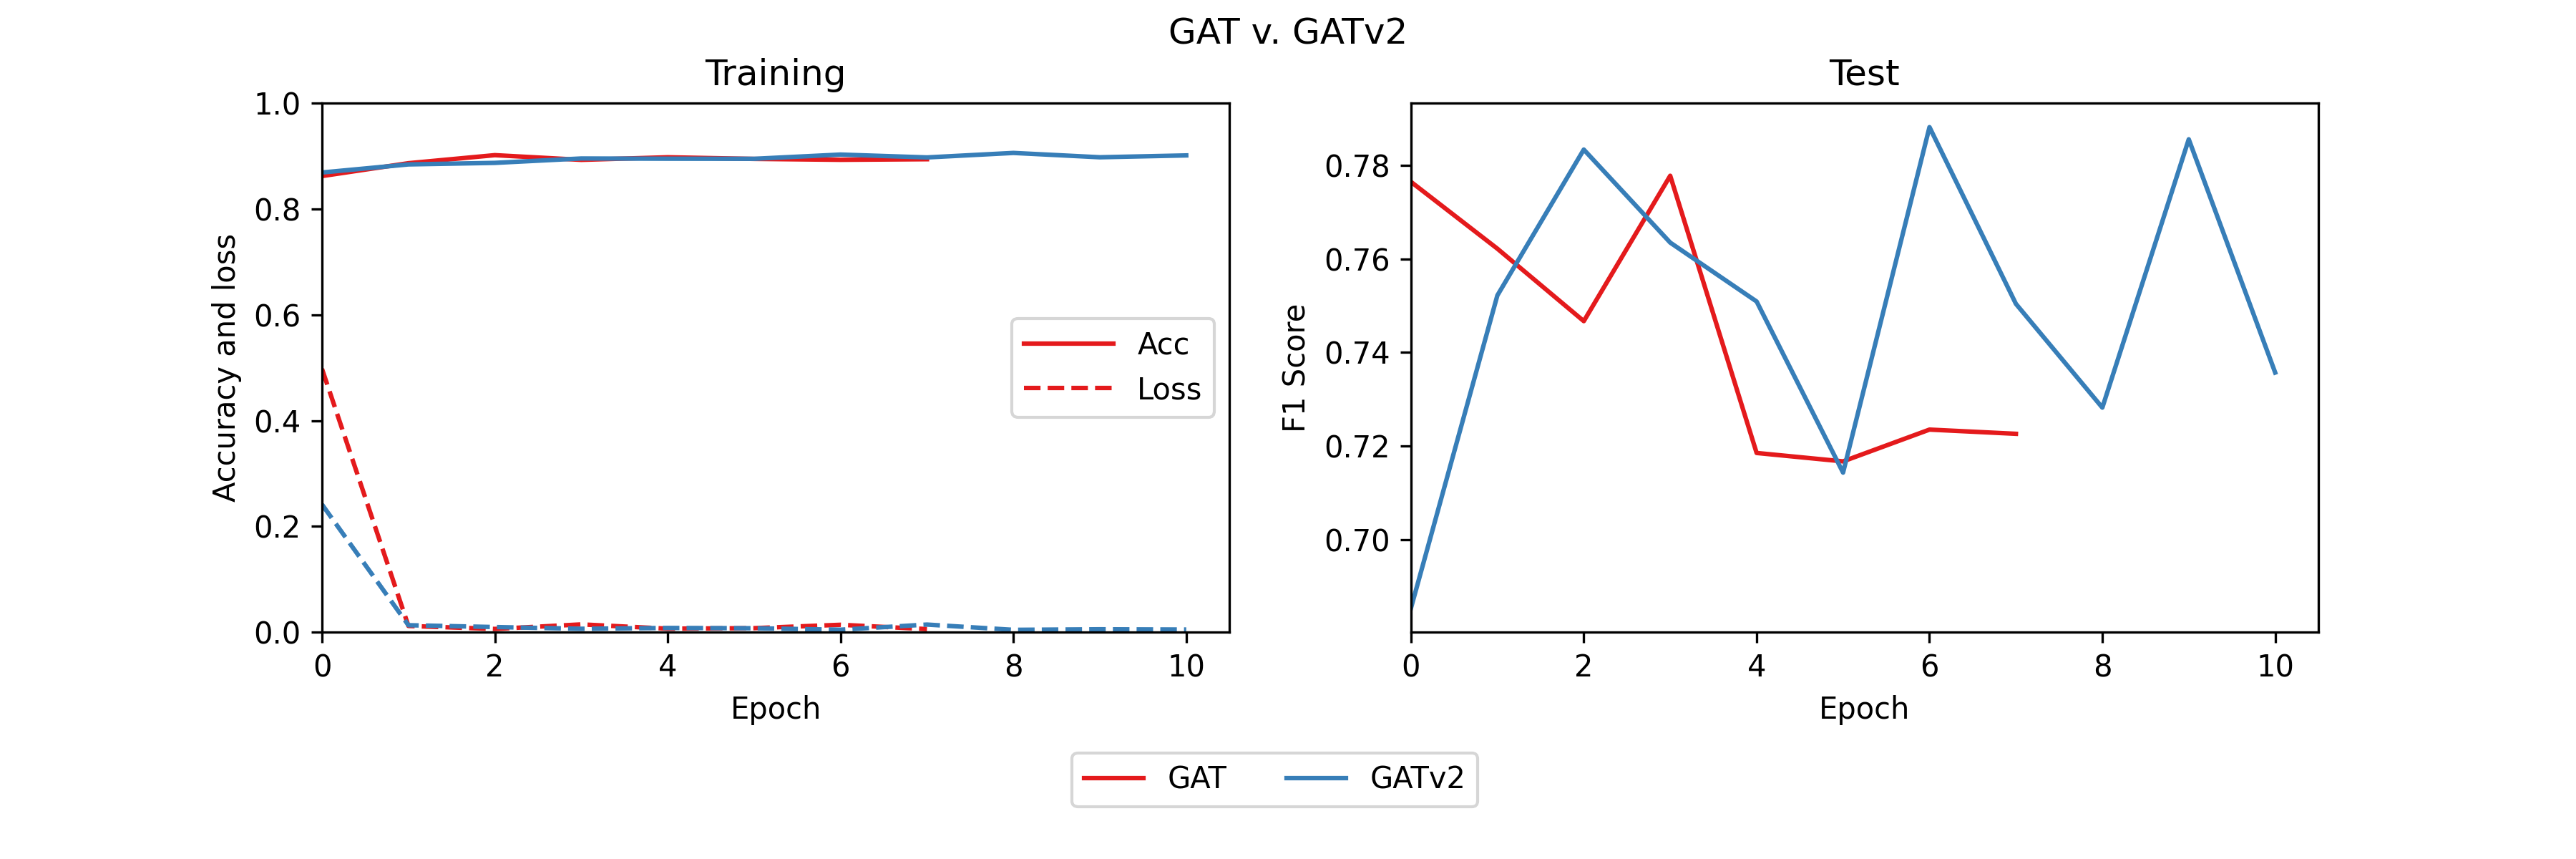
\includegraphics[width=\linewidth]{gat_v_gatv2.png}
    \caption{Comparison of model training accuracy, training loss and test F1 score for GAT and GATv2.}
\end{figure*}

Next, we trained each of our isolated bidirectional encoder models: BERT, RoBERTa and RoBERTa-RT. Due to RoBERTa's larger memory footprint, the RoBERTa models had to be trained with a batch size of 32, as compared to 64 for BERT. To compensate for this, we trained each RoBERTa model at a reduced learning rate compared to BERT following the square root rule \citep{Granziol2022}, e.g. reducing it from $5\times 10^{-5}$ to $3.5\times 10^{-5}$. All other hyperparameters were kept constant. As can be seen in Figure 3, all models converged quickly during training. Evaluating on the test data showed clear differences in the performance of the different models: BERT achieved an F1 score of 0.8481, RoBERTa 0.8518,\footnote{RoBERTa acutally performed slightly better (0.8547) with a learning rate of $5\times 10^{-5}$} RoBERTa-RT 0.8664.

\begin{figure*}[!h]
    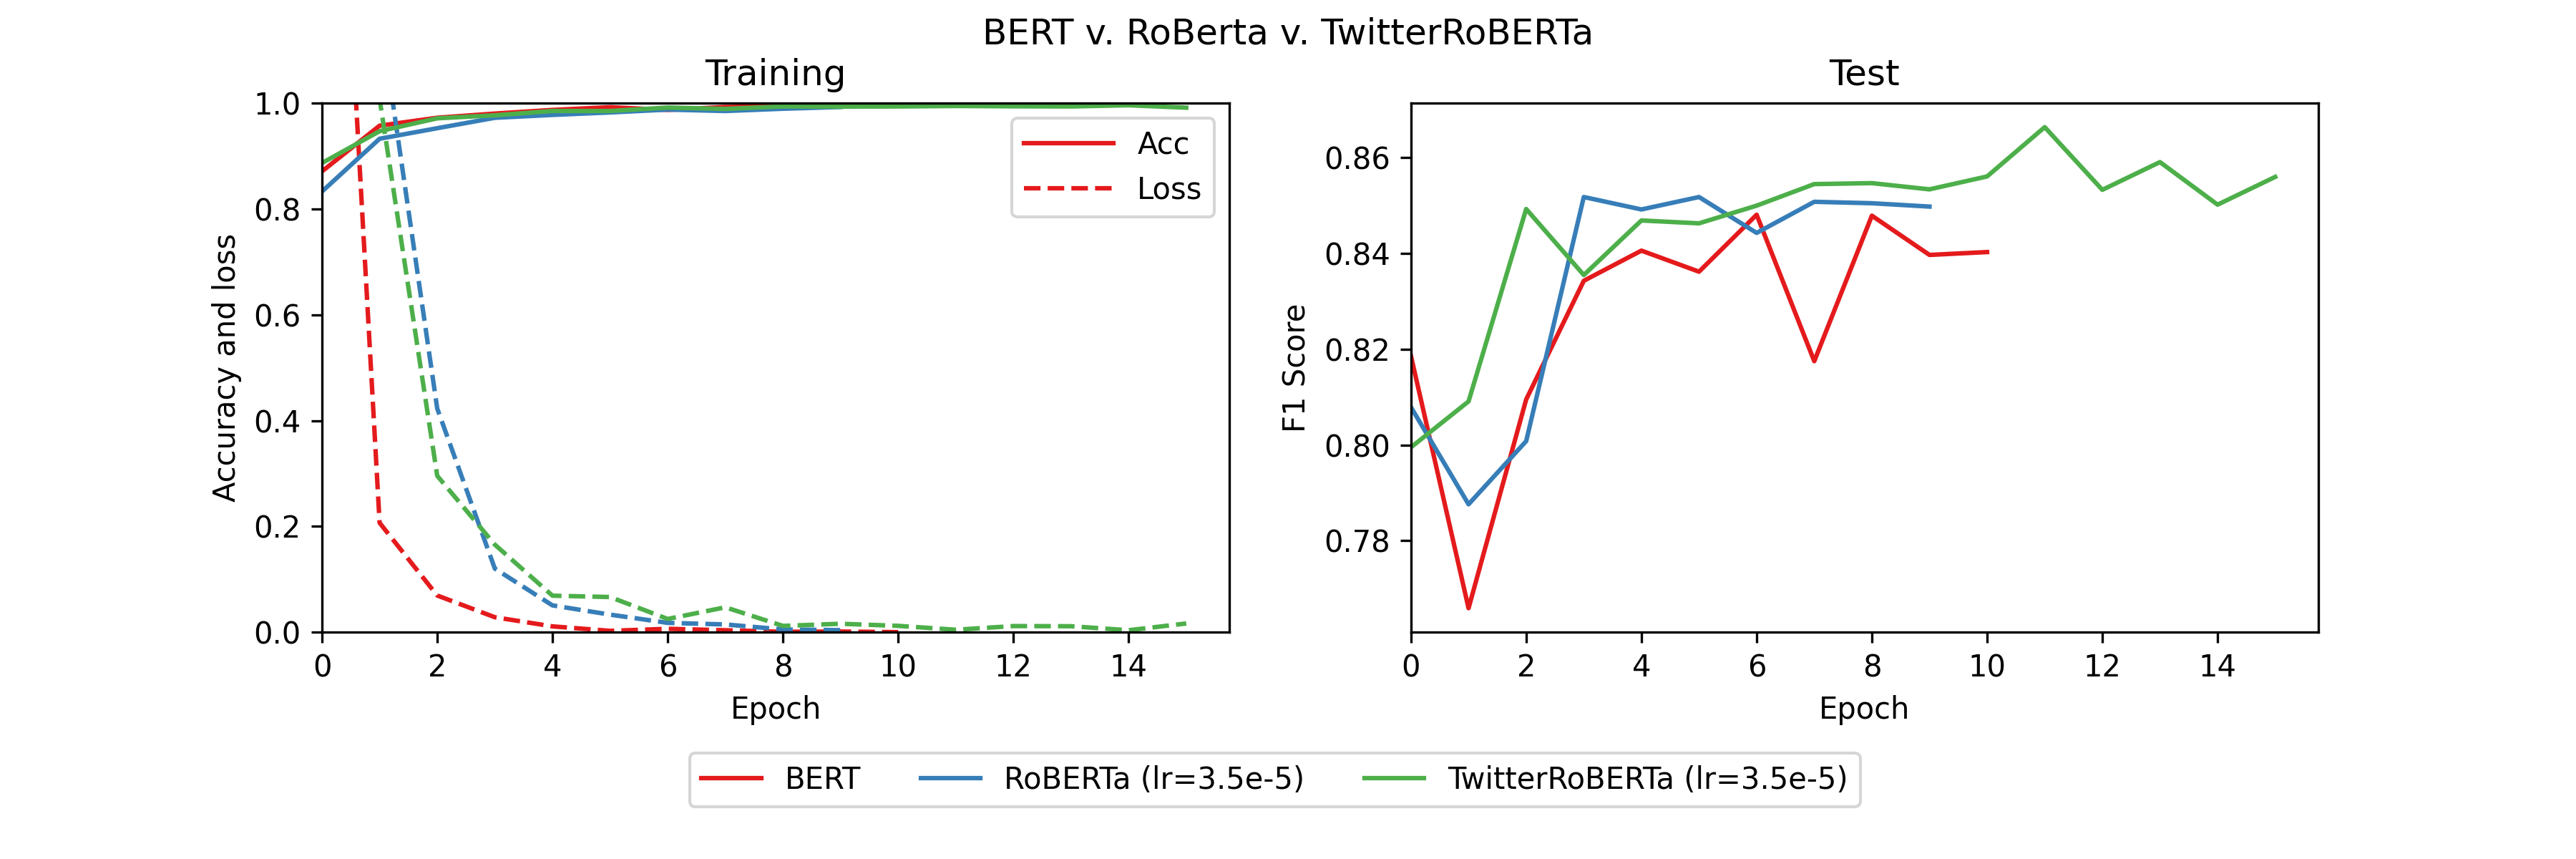
\includegraphics[width=\linewidth]{all_berts.png}
    \caption{Comparison of model training accuracy, training loss and test F1 score for BERT, RoBERTa and RoBERTa-RT.}
\end{figure*}

After demonstrating the improvements in isolation, we conduct several experiments to evaluate the incorporation of the different modules on the end-to-end models performance. For this, we initially trained 9 models in addition to our baseline. Each model was trained using the same hyperparameters except for the batch size and learning rate, for the reason mentioned previously: a batch size of 32 or 64 (depending on memory footprint), a learning rate of $1\times 10^{-2}$ for the graph attention layer, a learning rate of $5\times 10^{-5}$ or $3.5\times 10^{-5}$ for all other layers, a dropout rate of 0.5, a transformer attention dropout rate of 0.1, a transformer hidden dropout rate of 0.1, and a hidden vector size of 786. After running these initial experiments, we added two more versions of the GATv2+RoBERTa-RT model with a lower learning rate of $1\times 10^{-5}$ which led to slightly better performance on the test dataset for that particular architecture. The results of each models evaluation on the test dataset can be seen in Table 1. In comparison with our baseline, we can see that GATv2 in combination with the RoBERTa-based model outperform all other possible combinations suggesting that incremental improvements to the performance of the modules does have an impact on the performance of the end-to-end model. Table 2 shows an ablation showing the effect of modifying the graph attention module and Table 3 the effect of modifying the bidirectional encoder module.

\begin{table}
    \begin{tabular}{|c||c|c|c|c|}
        \hline
        Model & $bs$ & $lr$ & F1 score \\
        \hline 
        \hline
        GAT+BERT & 64 & $5\times10^{-5}$ &  0.8893 \\
        GAT+RoBERTa & 32 & $5\times10^{-5}$ &  0.8779 \\
        GAT+RoBERTa & 32 & $3.5\times10^{-5}$ &  0.8898 \\
        GAT+RoBERTa-RT & 32 & $5\times10^{-5}$  & 0.8934 \\
        GAT+RoBERTa-RT & 32 & $3.5\times10^{-5}$  & 0.8925 \\
        GATv2+BERT & 64 & $5\times10^{-5}$  & 0.8876 \\
        GATv2+RoBERTa & 32 & $5\times10^{-5}$ &  0.8968 \\
        GATv2+RoBERTa & 32 & $3.5\times10^{-5}$ &  \textbf{0.8983} \\
        GATv2+RoBERTa & 32 & $1\times10^{-5}$ &  0.8866 \\
        GATv2+RoBERTa-RT & 32 & $3.5\times10^{-5}$  & 0.8949 \\
        GATv2+RoBERTa-RT & 32 & $3.5\times10^{-5}$  & 0.8919 \\
        GATv2+RoBERTa-RT & 32 & $1\times10^{-5}$  & \textbf{0.8985} \\
        \hline
    \end{tabular}
    \caption{Selected combinations of different graph attention networks, language models and learning rates ($lr$), trained for 20 epochs with early stopping ($patience=5$). Batch size ($bs$) was only modified in order for the given model to fit in GPU memory.}
\end{table}

% \begin{figure*}[!h]
%     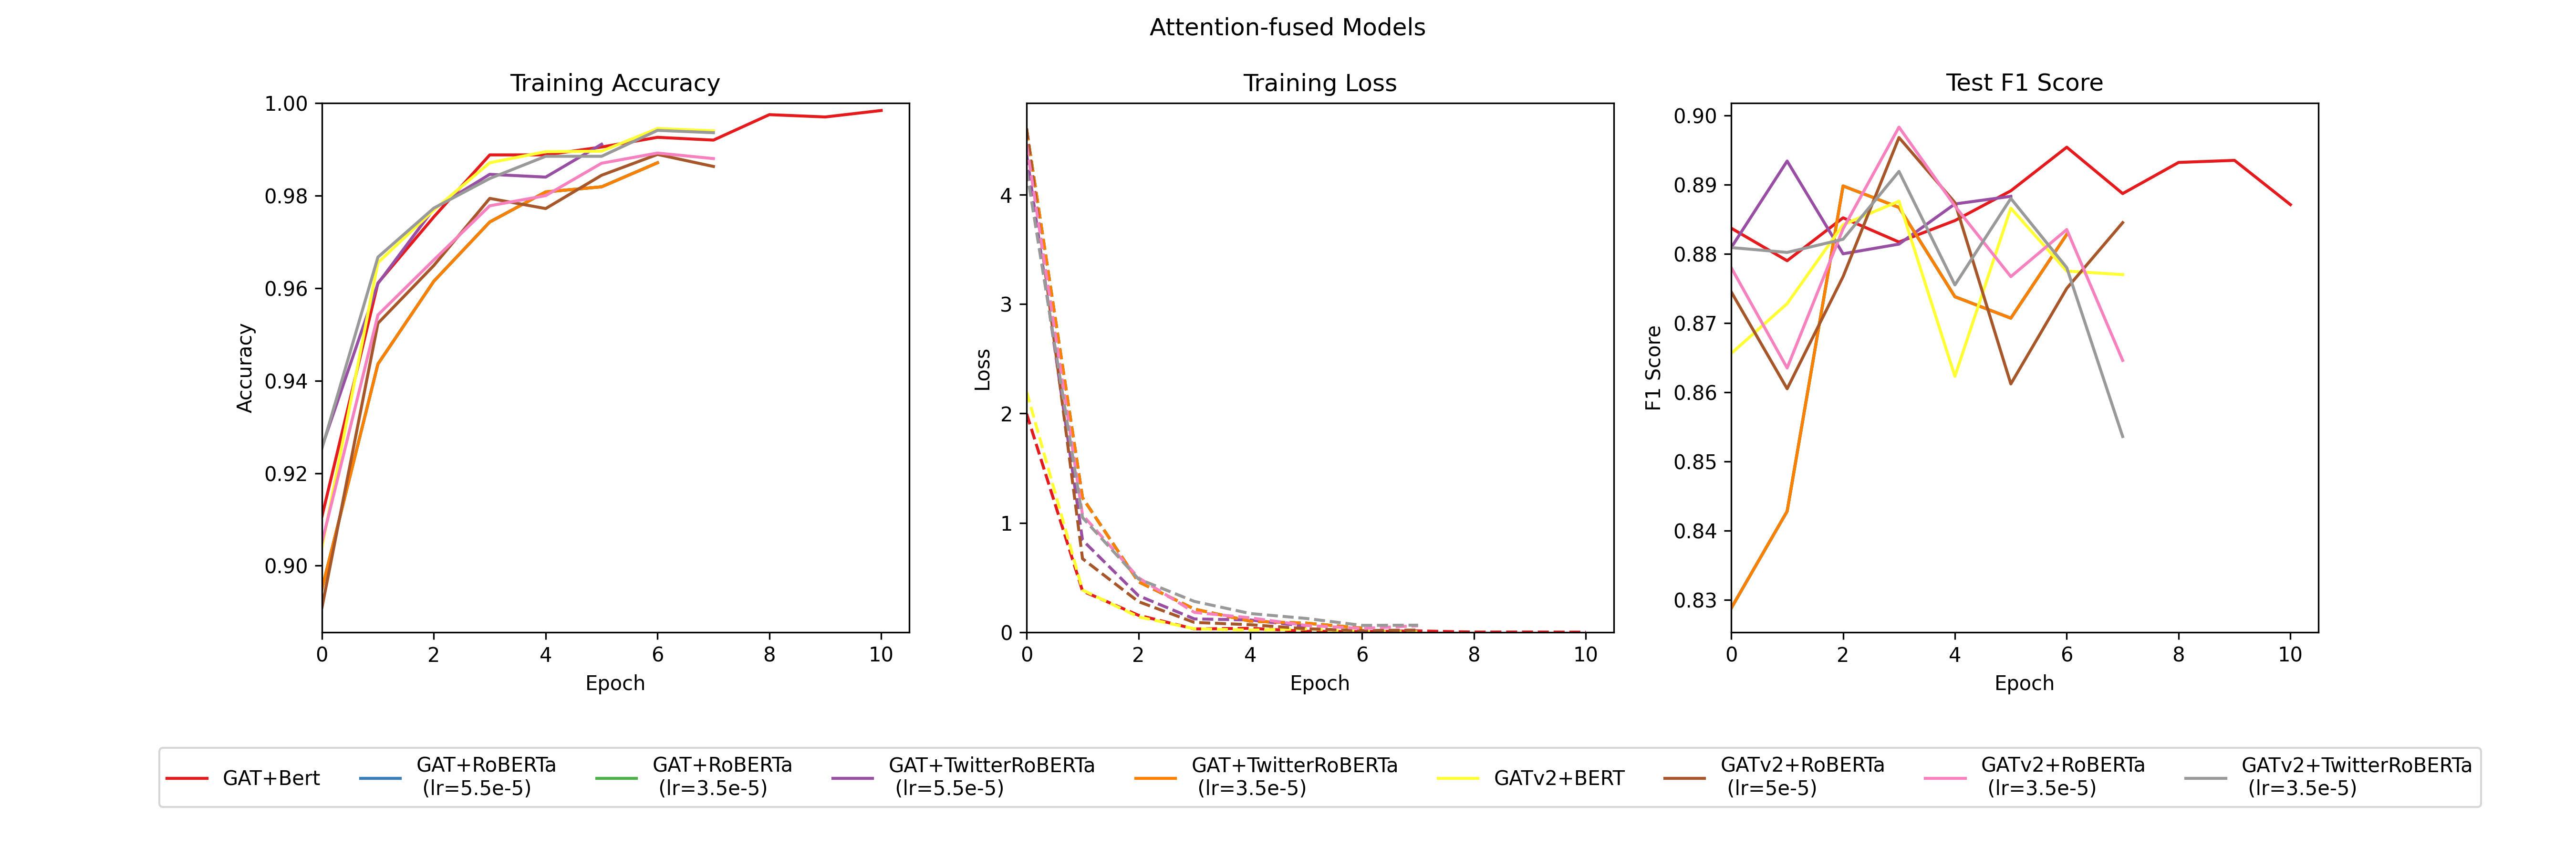
\includegraphics[width=\linewidth]{all_joint.png}
%     \caption{Comparison of model training accuracy, training loss and test F1 score for all attention-fused models.}
% \end{figure*}

\begin{table}
    \begin{tabular}{|c||c|c|c|c|}
        \hline 
        BERT module & BaseF1 & +GAT & +GATv2 & Diff \\
        \hline
        \hline
        None & n/a & 0.7778 & 0.7882 & +0.0104 \\
        BERT & 0.8481 & \textbf{+0.0512} &  +0.0395  & -0.0117 \\
        RoBERTa & 0.8547 & +0.0351 & \textbf{+0.0436} & +0.0085 \\
        RoBERTa-RT & 0.8664 & +0.0270 & \textbf{+ 0.0321} & +0.0051 \\
        \hline
    \end{tabular}
    \caption{Ablation showing additive value of GAT and GATv2 per base language model. The \textit{Diff} column is the difference between the increase attributed to the use of GAT and GATv2. As expected, the inclusion of a more expressive graph attention module leads to an increase in the end-to-end model's performance. }
\end{table}

\begin{table}
    \begin{tabular}{|c||c|c|c|}
        \hline
        GAT module & BERT (base) & RoBERTa & RoBERTa-RT  \\
        \hline 
        \hline
        None & 0.8481 & +0.0037 &  \textbf{+0.0183}  \\
        +GAT & 0.8893 & +0.0005 & \textbf{+0.0041} \\
        +GATv2 & 0.8876 & +0.0107 & \textbf{+0.0109} \\
        \hline
    \end{tabular}
    \caption{Ablation showing additive value of modifying the bidirectional encoder module. As would be expected, the inclusion of more expressive BERT modules leads to an increase in the end-to-end model's performance.}
\end{table}

\section{Results}

For our final results, we performed 10 iterations each for the baseline GAT+BERT architecture and the final GATv2+RoBERTa-RT architecture. The summary statistics in Table 2 show the mean $\pm$ standard deviation, maximum and minimum test F1 scores. The GATv2+RoBERTa-RT architecture outperforms the baseline \textit{on average} but only by a small margin (0.0009). The result is surprising given that both GATv2 and RoBERTa-RT, when evaluated independently, unambiguously outperform the modules they replace by 0.0104 and 0.0183. Thus, our findings are that, as implemented here, \textit{attention fusion does appear to carry forward some limited portion of the improved representations from preceding layers but with diminishing returns}. 

% \begin{figure}
%     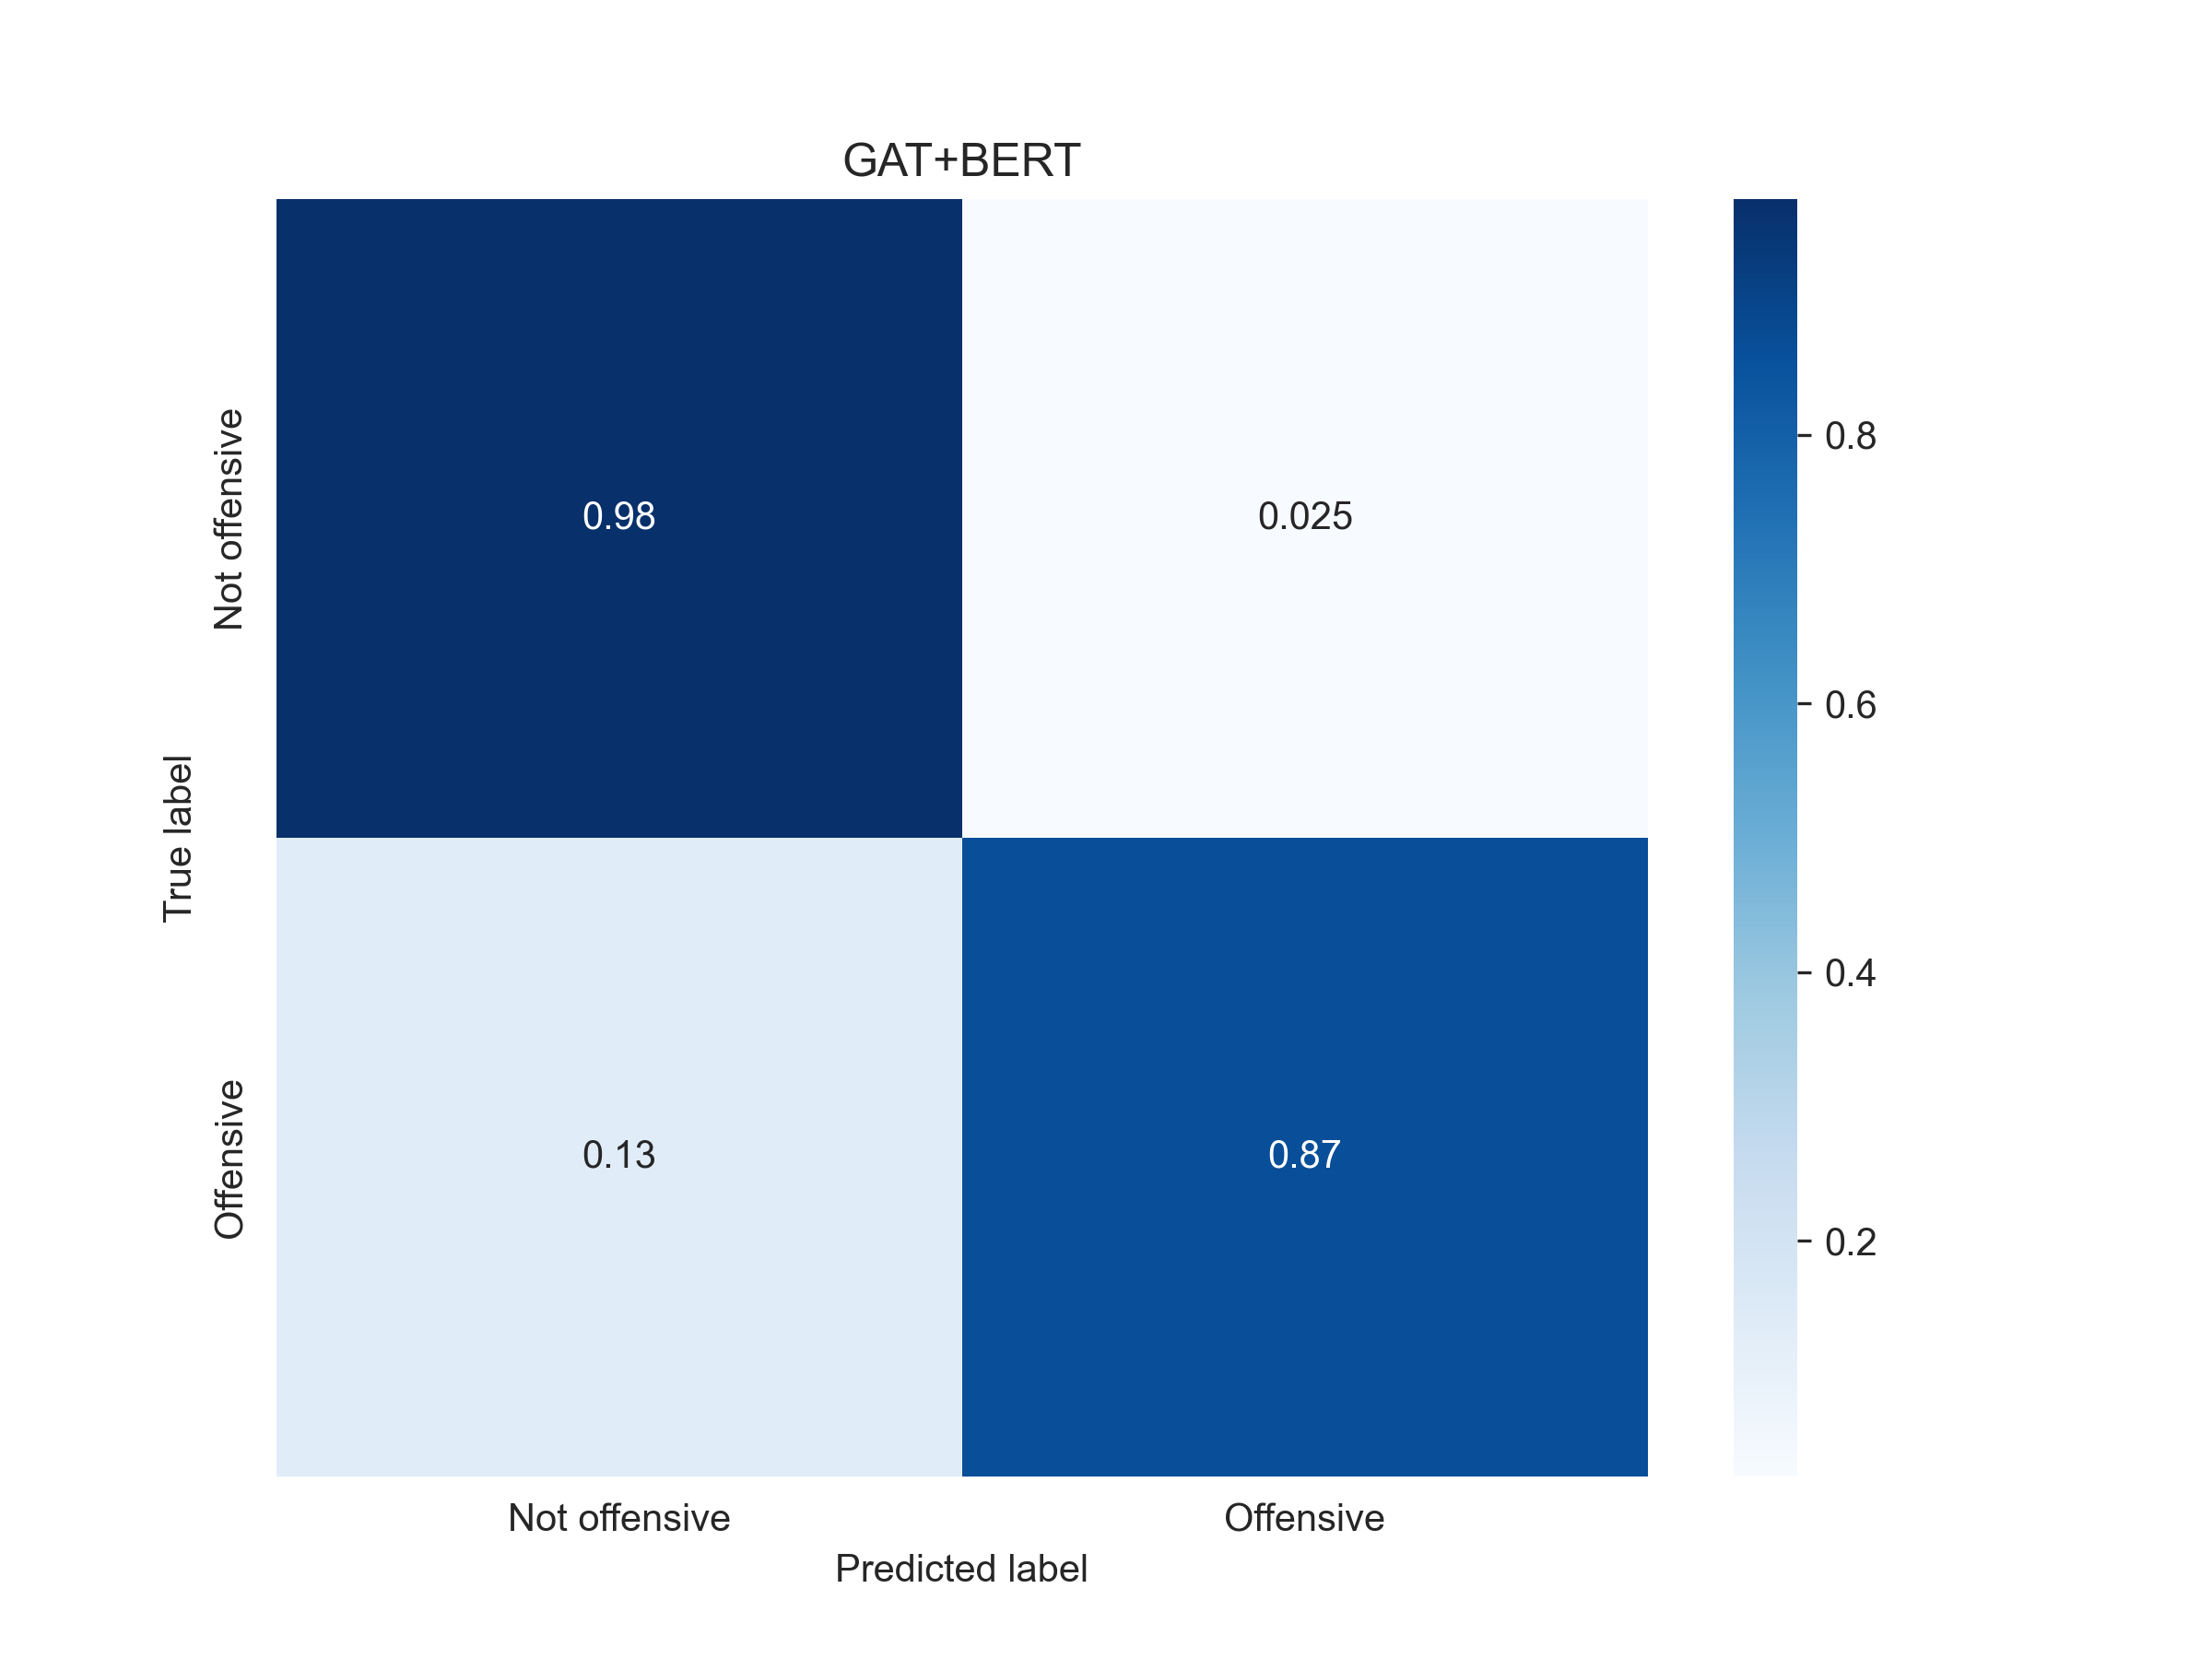
\includegraphics[width=\linewidth]{cm_baseline.png}
%     \caption{Confusion matrix for the baseline GAT+BERT model, normalized on true labels.}
% \end{figure}

\begin{figure}
    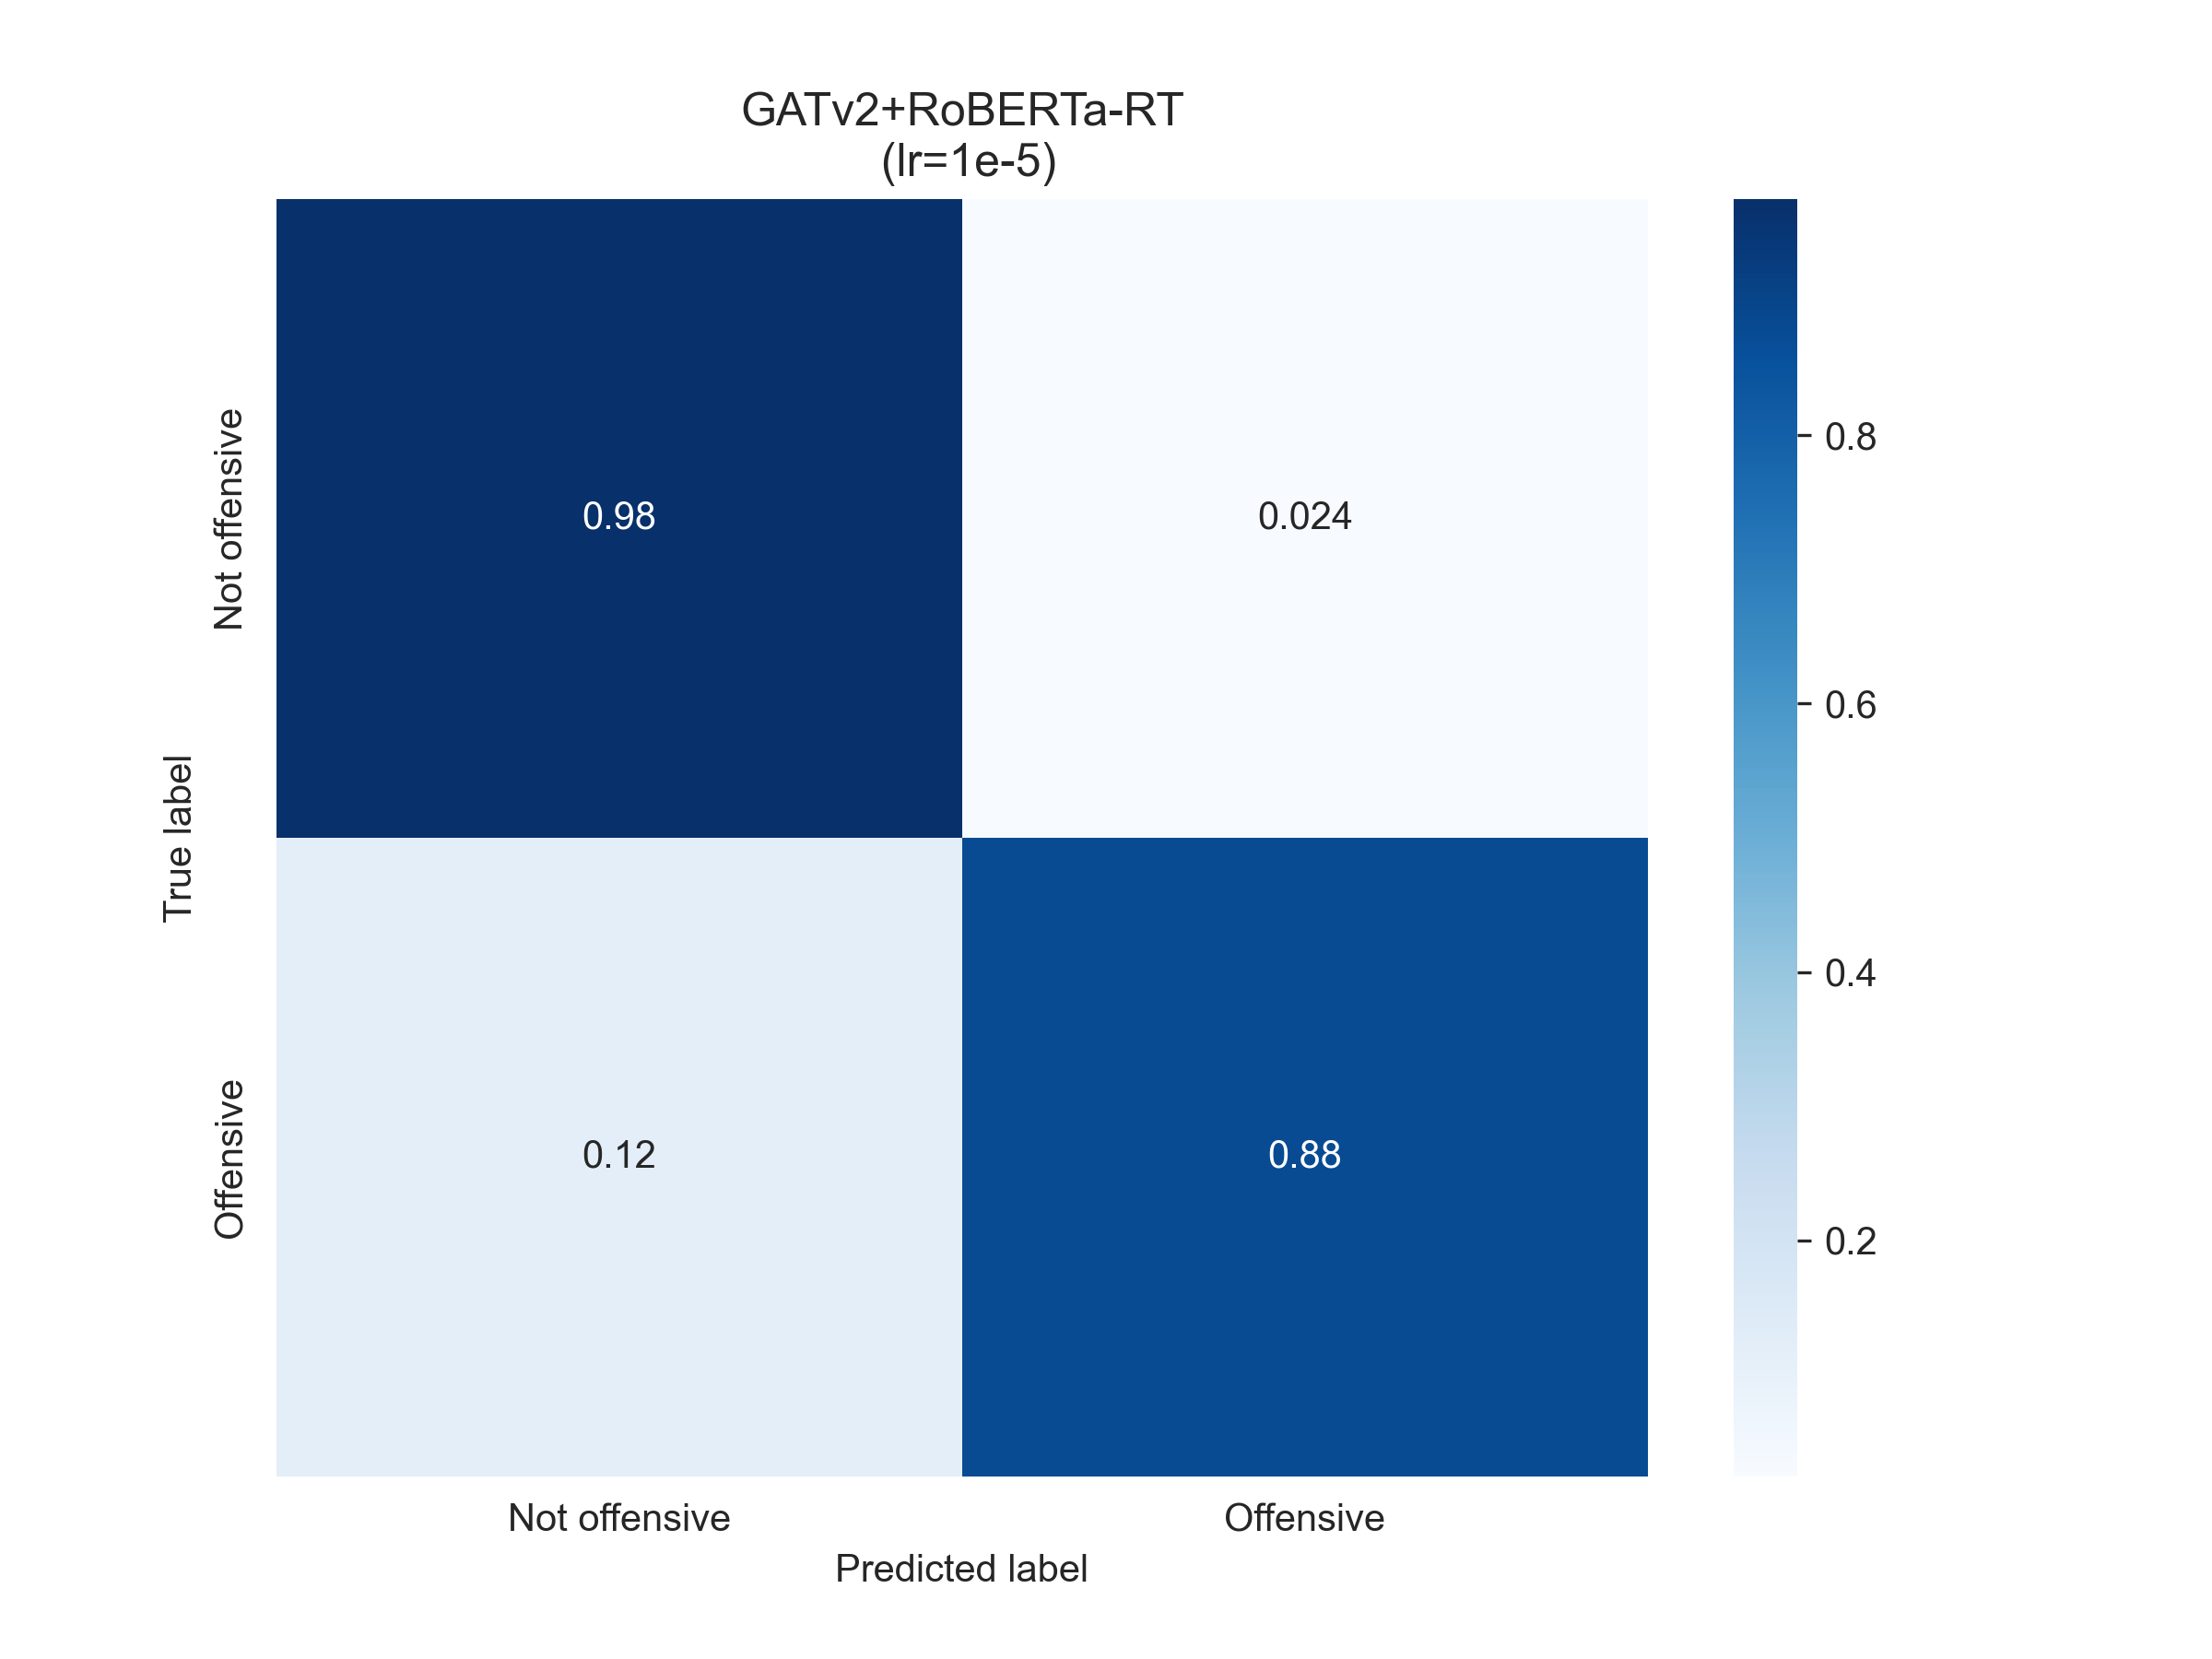
\includegraphics[width=\linewidth]{cm_final.png}
    \caption{Confusion matrix for the final GATv2+RoBERTa-RT model, normalized on true labels. Per-class accuracy of 0.98 and 0.88 on non-offensive and offensive labelled tweets, respectively.}
\end{figure}

\begin{table}
    \begin{tabular}{|c||c|c|c|}
        \hline
         & Baseline & Final  \\
         & GAT+BERT & GATv2 + RoBERTa-RT  \\
        \hline
        \hline 
        Mean F1  & $0.8927\pm0.0048$ & $\mathbf{0.8936 \pm 0.0047}$  \\
        Max F1 & \textbf{0.9018} & 0.9012 \\
        Min F1 & 0.7132 & \textbf{0.8230} \\
        \hline
    \end{tabular}
    \caption{Summary statistics for 10 iterations of the baseline GAT+BERT and final GATv2+RoBERTa-RT models.}
\end{table}

\section{Discussion}

Our results indicate that attention fusion appears to carry forward some improvements to representations introduced in preceding layers but with diminishing returns. For our discussion, we identify several avenues for further work and exploration. 

The first would be a more thorough comparison of models that incorporated hyperparameter tuning on a per-model basis, especially in regard to the application of different learning rates and regularization. At present, other than manually tuning the learning rate for the RoBERTa-based models to compensate for smaller batch sizes, we have not altered any of the model hyperparameters. Of special interest in this regard might be $\alpha$ and $\gamma$ parameters of the focal loss function as these directly relate to how much emphasis is given to the minority label in training. 

The second is to revisit the construction of the social graph and the derivation of the user embeddings to evaluate how well they are capturing community structure and explore how they could be improved. In particular, one could use non-parametric methods for community detection as a baseline against which to measure how effectively the graph attention layer is capturing community features. 

The third is a closer evaluation of attention fusion itself to see how it might be modified to better incorporate more expressive representations from preceding layers. For instance, what are the effects of increasing or decreasing the number of heads in the attention layer?

Lastly, but probably most significantly, do we just need more data? All the models we evaluated overfit the training dataset and, while performing well on the test set vis-\`a-vis other published results, do not generalize exceedingly well on a per-class basis. "More data" is generally a good strategy in such cases, but there are only a couple of Twitter datasets labelled for offensive language detection that include user information. For datasets that do not include user information, the retrieval of the missing information is possible but is often encumbered by the deletion of tweets and user accounts in the time since the dataset was originally collected \citep{Mishra2018}. Offensive language detection, and semantic analysis more generally, are amenable to data augmentation strategies, especially generation-based methods such as \citet{liu2020}. However, the end-to-end model described in this report would need to pair this with strategies for augmenting the graph-structured user data as well. While there are techniques for augmenting graph-structured data \citep{zhao2022}, a novel method for linking text and graph-structured data augmentation would need to be developed.

\appendix

\bibliography{project}

\end{document}